\section{Human Feature Analysis}\label{s:hfa}

% ============================================================
% WORD LIMITS: 1.1 = 100w, 1.2 = 100w, 1.3 = 100w
% EXCLUDED from count: equations, tables, figures, bibliography
% Examiners stop reading at the limit — cut ruthlessly.
% ============================================================

% ============================================================
\subsection{Human Patch Extraction}
% ============================================================
% TASK: adapt DL detection, propose lightweight useful-frame selection,
%       submit 50 patch samples. Evaluate. 100 words.
%
% SUGGESTED STRUCTURE (≈100 words — every word counts):
%   Sentence 1-2: method name, input, output.
%     "We apply YOLOv8m [CITE] to each training video, extracting
%      bounding-box crops of class `person' at every eligible frame."
%   Sentence 3-4: frame selection (the lightweight algorithm):
%     "To avoid redundant frames, we skip frames with inter-frame
%      mean absolute difference below \(\tau_{sc}=8\) (static shots)
%      and enforce a minimum spacing of 10 frames between YOLO calls.
%      Candidate patches are scored by a weighted combination of
%      detection confidence, relative bounding-box area (peak at 15\%
%      of frame), and Laplacian sharpness; greedy diversity sampling
%      then enforces a 10-frame temporal gap per video source."
%   Sentence 5: result.
%     "This yields 4,000 patches from 4 videos (2,000 game, 2,000 movie)."
%
% KEY THINGS TO JUSTIFY:
%   - Why YOLOv8? (SOTA, fast, pretrained on COCO persons)
%   - Why scene-change threshold? (avoids near-static shots)
%   - Why blur threshold differs? (film grain vs game rendering)
%   - Why greedy diversity? (prevents shot-repetition overfitting)
%   - State the extraction thresholds as concrete numbers
%
% EVALUATION (fits in ≤20 words + a figure):
%   - Quote the blur score range from _summary.txt: min 0.6, max 5351.5
%   - Quote how many raw detections → selected (10674 → 4000)
%
% FIGURES:
%   Fig 1a — 5×10 grid of sampled patches (50 required).
%             Sample script: randomly pick 50 from output/extracted_humans/20260314-195748/
%             Save to: paper/figs/patches_sample.pdf (or .png)
%             Caption: "Random sample of 50 extracted human patches."
%
%   Fig 1b (optional, fits in same figure with subcaption) —
%             Histogram of detection scores (before/after selection).
%             Source: output/extracted_humans/20260314-195748/_summary.txt
%             Save to: paper/figs/score_hist.pdf
%             Caption: "Score distribution of raw detections (grey) vs selected (blue)."
%             This gives you empirical justification for the scoring in ≤1 sentence.
%
% LATEX SKELETON:
% \begin{figure}[t]
%   \centering
%   \includegraphics[width=\linewidth]{figs/patches_sample.pdf}
%   \caption{Random sample of 50 extracted human patches from game (top two rows) and movie (bottom three rows) domains.}
%   \label{fig:patches}
% \end{figure}


\subsection{Classification}
% ============================================================
% TASK: classify 1.1 patches into 5 classes, submit 20/class.
%       Explain, justify, evaluate. 100 words.
%
% SUGGESTED STRUCTURE:
%   Sentence 1: define the 5 classes briefly.
%     "We define full-body as both hip keypoints visible with torso,
%      head-and-shoulder as upper body only, front/back by nose
%      visibility, and others for partial/occluded/non-human crops."
%   Sentence 2-3: method.
%     "We detect 17-point COCO keypoints with YOLOv8-pose [CITE],
%      then train a 3-layer Graph Convolutional Network (GCN)~\cite{kipf2017}
%      on the COCO skeleton graph with node features (x, y, confidence).
%      Confidence-weighted global pooling aggregates per-node embeddings
%      to a graph-level vector for 5-class classification."
%   Sentence 4: labels.
%     "Training labels are obtained from manual annotation of \(\sim\)600
%      patches using a custom Flask tool seeded with rule-based keypoint
%      heuristics."
%   Sentence 5: augmentation.
%     "Horizontal flip augmentation (swapping symmetric keypoint pairs)
%      doubles the training set without requiring additional annotations."
%   Sentence 6-7: result (refer to table/figure).
%     "Val accuracy: full-body-back 94.7\%, full-body-front 72.2\%,
%      head-shoulder-back 70.4\%, head-shoulder-front 65.3\%;
%      `others' accuracy is low (9.8\%), discussed below."
%
% KEY THINGS TO JUSTIFY:
%   - Why GCN over MLP/SVM? Pose is a graph structure — edges encode
%     skeletal connectivity; a GCN naturally propagates joint context.
%   - Why confidence-weighted pooling? Low-confidence keypoints
%     (occluded joints) should contribute less to the graph embedding.
%   - Why manual annotations? Rule-based heuristics misclassify
%     ambiguous poses; a brief ablation (training curves plot) shows
%     manual > rule.
%   - `others' failure: acknowledge it — this class is open-set
%     (no consistent pose signature), so low recall is expected.
%     Mitigation in 2.2: hard threshold on keypoint count.
%
% FIGURES:
%   Fig 2a — 4×5 grid of 20 patches per class (4 main classes × 5 each, or
%             20 per class across multiple figures).
%             Sample: randomly pick 20 from each subdir in
%             output/gcn_results/20260320-162455/<class>/
%             Save to: paper/figs/cls_samples_<class>.pdf
%             Tip: one combined figure with subcaptions per class saves space.
%
%   Fig 2b — GCN training curves (loss + accuracy over epochs).
%             Source: output/gcn_results/20260320-162455/training_curves.png
%             Copy to: paper/figs/gcn_training_curves.png
%             Caption: "GCN training and validation curves."
%
%   Table 1 — Per-class val accuracy (already in _summary.txt).
%             Present as a small table. Excluded from word count.
%             Columns: Class | Correct | Total | Accuracy (%)
%
% LATEX SKELETON:
% \begin{table}[t]
%   \centering
%   \caption{GCN per-class validation accuracy.}
%   \label{tab:gcn}
%   \begin{tabular}{lrrr}
%     \toprule
%     Class & Correct & Total & Acc.\ (\%) \\
%     \midrule
%     Full-body front    & 52 & 72  & 72.2 \\
%     Full-body back     & 18 & 19  & 94.7 \\
%     Head-shoulder front& 49 & 75  & 65.3 \\
%     Head-shoulder back & 19 & 27  & 70.4 \\
%     Others             &  5 & 51  &  9.8 \\
%     \bottomrule
%   \end{tabular}
% \end{table}


\subsection{Training Data Selection}
% ============================================================
% TASK: select most useful patches for style-transfer training.
%       Own observations/insights required. Submit 50 samples. 100 words.
%
% SUGGESTED STRUCTURE:
%   Sentence 1: observation / motivation.
%     "Inspection of extracted patches reveals substantial visual
%      redundancy: consecutive frames of the same shot produce
%      near-identical crops. Training CUT~\cite{park2020} on such
%      data risks overfitting the generator to specific shot compositions
%      rather than learning a domain-level style."
%   Sentence 2-3: method.
%     "We embed all non-`others' patches with DINOv2 ViT-B/14~\cite{oquab2023}
%      and apply K-Means independently within each class\,\(\times\)\,domain
%      group, allocating \(k \propto\) group size from a total budget of
%      2,000 patches.  The patch nearest (cosine distance) to each centroid
%      is selected as the most representative example."
%   Sentence 4: domain balance rationale.
%     "Processing game and movie groups independently preserves
%      the domain balance required by CUT's unpaired discriminator."
%   Sentence 5: result/figure reference.
%     "The resulting selection spans all pose classes and both domains;
%      Figure~\ref{fig:umap} confirms that DINOv2 clusters reflect
%      meaningful pose and domain variation."
%
% KEY THINGS TO JUSTIFY:
%   - Why DINOv2? Pretrained vision transformer captures high-level
%     semantic similarity better than pixel-level hashing or VGG features.
%     Cite: Oquab et al. (2023) DINOv2.
%   - Why per-(class × domain) independently? Maintains class and domain
%     balance for CUT; prevents majority-class clusters from absorbing
%     minority-class patches.
%   - Why centroid-nearest? Selects the most "typical" example in each
%     visual cluster rather than a random member.
%   - Caveat: DINOv2 trained on natural images — embedding may not
%     perfectly separate game-domain styles (worth one sentence).
%
% FIGURES:
%   Fig 3a — UMAP (already generated by the pipeline).
%             Source: figures/dino_umap.png
%             Copy to: paper/figs/dino_umap.png
%             Caption: "UMAP of DINOv2 patch embeddings: (left) coloured by class,
%                       (right) coloured by domain. Clusters reflect pose and domain
%                       variation, justifying embedding-based deduplication."
%             This is your key empirical evidence for 1.3.
%
%   Fig 3b — 50 selected sample patches (required submission).
%             Sample randomly from train_game + train_movie output of
%             select_with_dino_clustering.
%             Save to: paper/figs/selected_patches_sample.pdf
%
%   Optional: 2×2 grid showing a near-duplicate cluster (before deduplication)
%             vs. the selected centroid patch. Powerful visual argument.
%             Save to: paper/figs/dedup_example.pdf
%
% LATEX SKELETON:
% \begin{figure}[t]
%   \centering
%   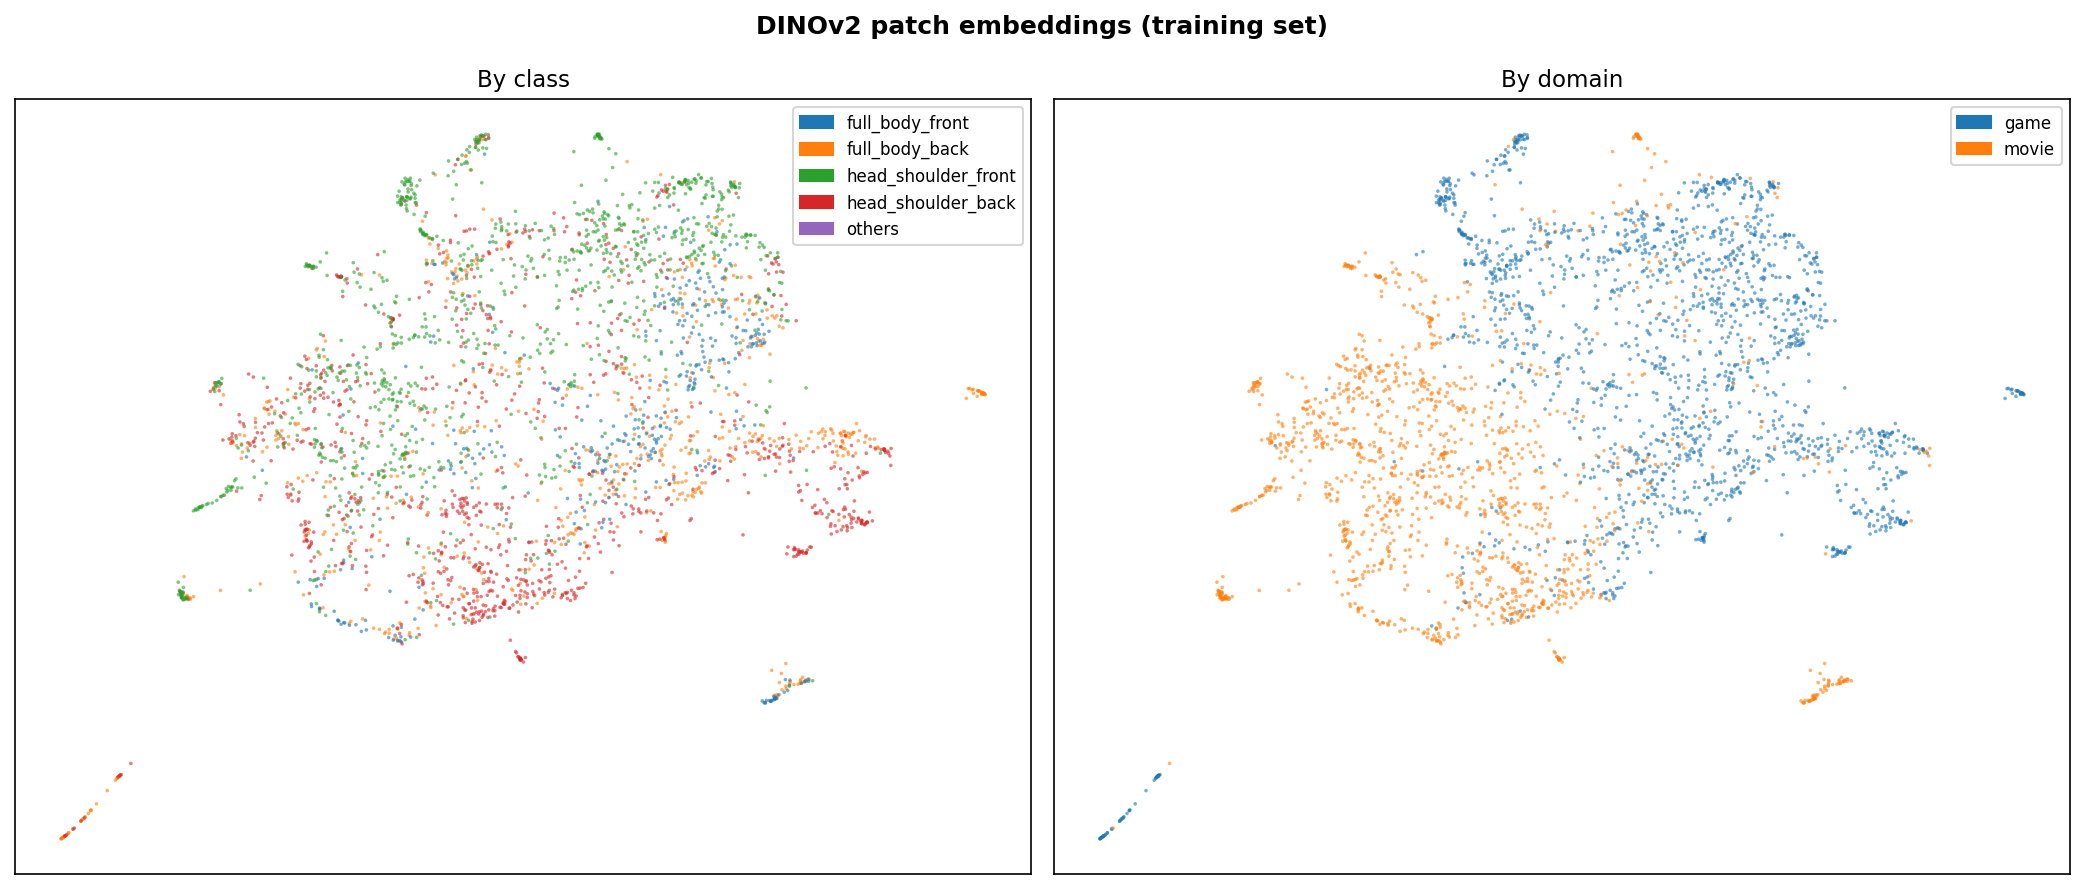
\includegraphics[width=\linewidth]{figs/dino_umap.png}
%   \caption{UMAP projection of DINOv2 embeddings for all training patches,
%            coloured by pose class (left) and domain (right). Clear clustering
%            motivates diversity-preserving selection.}
%   \label{fig:umap}
% \end{figure}
